\chapter{Theory}

\section{Processes}

As a unified formalism to describe many classes of infinite state systems,
process rewrite systems were introduced by \cite{Mayr00}.
They specify rewrite rules on processes as the states of the system.
The syntax here is taken from \cite{Esparza01}.

% processes are parallel or sequential

\begin{definition}[Process]
The set of \emph{processes} $\mc P$ over a set of
constants $Const = \{X,Y,…\}$ is given by
\begin{mathpar}
  \inferrule{ }{ε ∈ \mc P}\, (0) \hspace{1cm}
  \inferrule{X ∈ Const}{X ∈ \mc P}\, (1) \hspace{1cm}
  \inferrule{p ∈ \mc P \\ q ∈ \mc P}{p⋅q ∈ \mc P}\, (S) \hspace{1cm}
  \inferrule{p ∈ \mc P \\ q ∈ \mc P}{p\|q ∈ \mc P}\, (P)
\end{mathpar}
where $ε$ is the empty process, $X ∈ C$ are process constants,
$⋅$ means sequential composition and
$\|$ means parallel composition. 

Processes are considered equivalent under the smallest congruence relation
such that the operator $⋅$ is associative,
$\|$ is associative and commutative and
$ε$ is a unit for both $⋅$ and $\|$.

The class of processes just obtained with rule 0,1 and S are called sequential
processes, while processes just obtained with rule 0,1 and P are called
parallel processes.

From here on lowercase letters $p,q,…$ will denote any process, while
uppercase letters $P,Q,…$ will denote single process constants.
\end{definition}

\begin{example}
  The state of a pushdown automaton, given by a control state $P$ and
  a stack $A_1A_2 … A_n$, where $A_1$ is the top of the stack, can be given by a
  sequential process $P⋅A_1⋅A_2⋅…⋅A_n$.
  As an intuition, a transition from $P$ with the symbol $a$ to $Q$, by
  replacing $A_1$ on the stack with $B_1B_2$, could be given by
  a rewrite rule $P⋅A_1 \must[a] Q⋅B_1⋅B_2$. Applying this
  rule on the state yields $Q⋅B_1⋅B_2⋅A_2⋅…⋅A_n$. The formal definition for
  rewrite rules is given later.
\end{example}

\begin{definition}[Size of a process]
  The \emph{size} $|p|$ of a process $p$ is defined by
  \begin{align*}
    |ε| &= 0 \\
    |X| &= 1 \\
    |p⋅q| &= |p| + |q| \\
    |p \| q| &= |p| + |q|
  \end{align*}
  which is equal to the number of constants appearing in the process.
\end{definition}

\section{Modal transition system}

Modal transition systems and subsequently modal refinement are defined here as in \cite{BenesK12}.

\begin{definition}[Modal transition system]
A \emph{modal transition system (MTS)} over an action alphabet $Act = \{a, b, …\}$ is
a triple $(\mc P, \may[], \must[])$, where $\mc P$ is a set of processes and
$\must[] ⊆ \may[] ⊆ \mc P × Act × \mc P$.
An element $(p,a,q) ∈ \may[]$ is a \emph{may transition}, written as $p \may[a] q$,
and an element $(p,a,q) ∈ \must[]$ is a \emph{must transition}, written as $p \must[a] q$.
\end{definition}

When using the term of a process in the context of an MTS,
we will have its meaning include the underlying transition system.
That way we can talk about refinement of a process by another process
in the context of their originating systems.

\section{Modal refinement}

\begin{definition}[Refinement]
  Let $(\mc P, \may, \must)$ be an MTS and $p,q ∈ \mc P$ be processes.
  We say that $p$ \emph{refines} $q$, written as $p ≤_m q$, if there is a relation
  $\mc R ⊆ \mc P × \mc P $ such that
  $(p, q) ∈ \mc R$ and for every $(p, q) ∈ \mc R$ and every $a ∈ Act$:
  \begin{enumerate}
    \item If $p \may[a] p'$ then there is a transition $q \may[a] q'$ s.t.
          $(p',q') ∈ \mc R$.
    \item If $q \must[a] q'$ then there is a transition $p \must[a] p'$ s.t.
          $(p',q') ∈ \mc R$.
  \end{enumerate}
\end{definition}

Out of simplicity, we only regard refinement for two processes from a single MTS.
Modal refinement of processes from two different MTS can be reduced to this by taking
the disjoint union of the MTS.

The intuition for a process $p$ refining another process $q$ is that
$p$ is more specific than $q$, while $q$
is more abstract than $p$.
Modal refinement can then be used to compare different specifications
of a system or to obtain an \emph{implementation}, that is
an MTS with $\may[] = \must[]$.

Modal refinement can also be seen as a refinement game, similar to
the standard simulation or bisimulation game \cite{Srba06}.
The states of the game are pairs of processes $(p,q)$,
and in each round a process from one side
plays an attacking transition, to which the other process
answers with a defending transition.
This leads to a new state, from which the game continues.
The attacker wins if at some state the defender can not play any more transitions,
otherwise the defender wins.

An \emph{attacking transition} from the state $(p,q)$ is any
transition of the form $p \may[a] p'$ or $q \must[a] q'$.
Given that attacking transition, any transition of the form
$q \may[a] q'$ or $p \must[a] p'$ matching the action and the
transition type is a \emph{defending transition}.
That choice of transitions then leads to the state $(p',q')$.

Then $p ≤_m q$ holds if and only if
there is no winning strategy for the attacker from $(p,q)$, i.e.
a sequence of attacking transitions such that for every choice of defending transition,
a state $(p',q')$ is reached from which there is an attacking transition but no
defending transition. The complete characterization for this is given in \cite{BenesK12}.

\section{Modal process rewrite system}

Modal process rewrite systems are defined here as
a straightforward extension of
process rewrite systems \cite{Mayr00, Esparza01},
with their modal subclasses defined analogously.

\begin{definition}[Modal process rewrite system]
A \emph{process rewrite system (PRS)} over an action alphabet $Act$
is a finite relation $Δ ⊆ \mc P ∖ \{ε\} × Act × \mc P$.
Elements of $Δ$ are called \emph{rewrite rules}.
A \emph{modal process rewrite system (mPRS)} is a tuple $(\Dmay, \Dmust)$ where
$\Dmay, \Dmust$ are process rewrite systems such that $\Dmay ⊆ \Dmust$.

An mPRS $(\Dmay, \Dmust)$ induces an MTS $(\mc P, \may[], \must[])$ as follows:
\begin{mathpar}
  \inferrule{(p, a, p') ∈ \Dmay}{p \may[a] p'} \, (1) \quad
  \inferrule{(p, a, p') ∈ \Dmust}{p \must[a] p'} \, (2) \\
  \inferrule{p \may[a] p'}{p⋅q \may[a] p'⋅q} \, (3) \quad
  \inferrule{p \must[a] p'}{p⋅q \must[a] p'⋅q} \, (4) \quad
  \inferrule{p \may[a] p'}{p\|q \may[a] p\|q} \, (5) \quad
  \inferrule{p \must[a] p'}{p\|q \must[a] p'\|q} \, (6)
\end{mathpar}
\end{definition}

\section{Visibly pushdown automaton}

Visibly pushdown automata are a subclass of
PDA that partition
their action alphabet into call actions,
internal actions and return actions.
Here they will be represented by a PRS in
the same form used to represent PDA.

\begin{definition}[Visibly pushdown automaton]
A PRS $Δ$ over the action alphabet $Act$ is a
\emph{visibly pushdown automaton (vPDA)} if
there is a partition
$Act = Act_r \uplus Act_i \uplus Act_c$
such that every rule $(p, a, p') ∈ Δ$ has the form
\begin{align*}
  p &= P⋅S
  & &\text{and} &
  p' &= \begin{cases}
  Q & \text{if } a ∈ Act_r \quad \text{(return rule)}\\
  Q⋅T & \text{if } a ∈ Act_i \quad \text{(internal rule)} \\
  Q⋅T⋅R & \text{if } a ∈ Act_c \quad \text{(call rule)}
\end{cases}
\end{align*}
for some $P,Q,S,T,R ∈ Const$.
A \emph{modal visibly pushdown automaton (mvPDA)} is an
mPRS $(\Dmay, \Dmust)$ such that $\Dmay$ and $\Dmust$ are vPDA with
the same action alphabet partition.
\end{definition}

The rules of a vPDA are called return rules if they pop a symbol
from the stack, internal rules if they only change the top symbol
or call rules if they push a symbol to the stack.
A vPDA always makes the type of rule used visible through the
action. In contrast to a PDA, this means that two vPDA
performing the same actions will always have the same number
of symbols on the stack. This will be crucial to decide
refinement between them.

We will have a look at the concepts introduced so far in an example.

\begin{example}
  Suppose we have a modular specification for a vending machine
  that can offer either tea, coffee, or both.
  They should only be offered after inserting coins, although that is optional.
  However after inserting a number of coins, the machine either has to offer
  one tea for each coin inserted or one coffee for each coin inserted.
  It may also offer the other type of beverage, but does not need to.
  Then we obtain a proposed implementation and want to test if it refines
  the specification.
  
  Figure \ref{fig:vending-mvpda} shows both implementation and specification modeled by
  an mvPDA. Note that may transitions are implied by the must transitions.

  The process $Q⋅S$ on the right is the specification. 
  After inserting the first coin, the machine
  non-deterministically chooses either tea or coffee by pushing $T$ or $C$
  on the stack. This symbol is added for every additional coin.
  It can be popped for the chosen beverage and may also be popped for the
  other one.
  
  The process $P⋅S$ on the left is the implementation.
  It avoids non-determinism, so after inserting
  coins it just stores that information on the stack with the symbol $M$.
  When it offers a beverage, it locks in the chosen type by either going to
  the state $T$ or $C$. From those states it can only offer the chosen beverage,
  until no more coins are left.
\end{example}

\begin{figure}[ht]
  \centering
  \begin{minipage}[b]{.45\textwidth}
    \begin{align*}
      P⋅S &\must[coin] P⋅M⋅S \\
      P⋅M &\must[coin] P⋅M⋅M \\
      C⋅S &\must[coin] P⋅M⋅S \\
      T⋅S &\must[coin] P⋅M⋅S \\
      P⋅M &\must[tea] T \\
      P⋅M &\must[coffee] C \\
      T⋅M &\must[tea] T \\
      C⋅M &\must[coffee] C
    \end{align*}
  \end{minipage}\quad
  \begin{minipage}[b]{.45\textwidth}
    \begin{align*}
      Q⋅S &\may[coin] Q⋅T⋅S \\
      Q⋅S &\may[coin] Q⋅C⋅S \\
      Q⋅T &\may[coin] Q⋅T⋅T \\
      Q⋅C &\may[coin] Q⋅C⋅C \\
      Q⋅T &\must[tea] Q \\
      Q⋅T &\may[coffee] Q \\
      Q⋅C &\may[tea] Q \\
      Q⋅C &\must[coffee] Q
    \end{align*}
  \end{minipage}
  \caption{Vending machine mvPDA}
  \label{fig:vending-mvpda}
\end{figure}
  
\begin{example}
  We can look at some refinement problems on the mvPDA from figure \ref{fig:vending-mvpda}.
  First we want to decide if $T⋅M ≤_m Q⋅T$ holds.
  From $T⋅M$, the only may transition possible is $T⋅M \may[tea] T$, which is answered
  by $Q⋅T \may[tea] Q$. From $Q⋅T$, the only must transition is $Q⋅T \must[tea] Q$,
  which is answered by $T⋅M \must[tea] T$. In both cases there are no more
  transitions from the resulting state $(T,Q)$, therefore $T⋅M ≤_m Q⋅T$ holds.

  On the other hand, $C⋅M ≤_m Q⋅T$ does not hold, as from $Q⋅T$ there is the transition
  $Q⋅T \must[tea] T$, but there is no transition of the form $C⋅M \must[tea] p'$.

  The main problem is to decide whether $P⋅S ≤_m Q⋅S$ holds. It is not easy to see
  if it does from the rules directly.
  However later we will construct a method to decide it algorithmically
  and show that it actually does not hold.
\end{example}

\section{Attack tree}

When regarding refinement as a game, the strategies for the attacker can be seen
as trees. That will be done through attack trees, as a representation of partially
or fully explored strategies. These can then be used to decide refinement.

\begin{definition}[Attack tree]

  An \emph{attack tree} over a set of processes $\mc P$ is a rooted tree where
  each node has two kinds of children, child states and child trees.
  It is given by a triple $((p,q),O,C)$,
  representing the tree with the root node labeled by $(p,q) ∈ \mc P^2$,
  the set of open edges $O$ leading to child states $(p',q') ∈ \mc P^2$ and
  the set of closed edges $C$ leading to the attack trees that are children of the
  root node.
  
  For an attack tree $T = ((p,q),O,C)$, we will use the short notations
  $T_r = (p,q)$ for the label of the root, $T_O = O$ for the set of child states
  and $T_C = C$ for the set of child trees.
  
  The set of attack trees $\mc T$ constructible from an MTS $(\mc P, \may, \must)$
  is defined by:
  \begin{mathpar}
    \inferrule{p,q ∈ \mc P, p \may[a] p'}
      {((p,q), \{ (p', q') \mid q \may[a] q' \}, ∅) ∈ \mc T}
    \, (1) \\
    \inferrule{p,q ∈ \mc P, q \must[a] q'}
      {((p,q), \{ (p', q') \mid p \must[a] q' \}, ∅) ∈ \mc T}
    \, (2) \\
    \inferrule{T ∈ \mc T \\ R ∈ \mc T \\ R_r ∈ T_O}
      {(T_r, T_O ∖ \{R_r\}, T_C ∪ \{R\}) ∈ \mc T}
    \, (3) \\
  \end{mathpar}
  
  Rules 1 and 2 construct an initial tree for an attacking transition with edges to
  states for each possible defending transitions,
  while rule 3 replaces an open edge to a state with a tree having that state as the
  label of its root.

  As we can see from the construction rules, every node in a tree
  has a corresponding attacking transition, while for each edge from that node
  there is an applicable defending transition.
  Similarly, as the total number of edges never changes, there is an edge
  for each applicable defending transition.
  Therefore nodes can be identified with attacking transitions and edges with
  defending transitions.

  For an attack tree $T$, the set of all \emph{subtrees} of $T$,
  including $T$ itself, is given recursively by
  $subtree(T) = T ∪ \left(⋃_{T' ∈ T_C} subtree(T') \right)$.
  
  The set of all \emph{open states} of $T$ are the child states that
  have an open edge to it, that is $open(T) = ⋃_{T' ∈ subtree(T)} T'_O$
  or equivalently $open(T) = T_O ∪ \left(⋃_{T' ∈ T_C} open(T') \right)$.
  
  A tree is said to be \emph{closed} if it has no open states, that is
  $closed(T) \iff open(T) = ∅$.
\end{definition}

The construction rules for attack trees only allow us to add a tree
as a subtree from an open state in the root node.
However, the following lemma shows that any open states in the tree
can be replaced by a matching tree.

\begin{lemma}[Tree composition]
  \label{lemma:tree-composition}
  If there are attack trees $T$ and $R$ with
  $R_r ∈ open(T)$,
  then there is an attack tree $S$ with
  $S_r = T_r$ and
  $open(S) = open(T) ∖ \{R_r\} ∪ open(R)$.
\end{lemma}
\begin{proof}
  We prove the proposition by induction on the number of proper subtrees
  with an open edge to $R_r$, that is
  $n = |\{ T' ∈ subtree(T) \mid T' ≠ T ∧ R_r ∈ open(T')\}|$:
  \begin{enumerate}
    \item $n = 0$:
      Then $R_r ∈ T_O$ and $R_r ∉ open(T')$ for $T' ∈ T_C$,
      so with rule 3 we can construct
      $S = (T_r, T_O ∖ \{R_r\}, T_C ∪ \{R\})$ with
      $open(S) = open(T) ∖ \{R_r\} ∪ open(R)$.
    \item $n ≥ 1$:
      Then there is $T' ∈ T_C$ such that $R_r ∈ open(T')$.
      $T'$ does not have itself as a proper subtree
      with an open edge to $R_r$, so we can apply
      the induction hypothesis to obtain
      $S'$ with $S'_r = T'_r$ and
      $open(S') = open(T') ∖ \{R_r\} ∪ open(R)$.

      As $T'$ was added to $T_C$ some point in the construction of $T$,
      we can substitute $T'$ with $S'$ at that point and obtain
      $T''$ with $T''_r = T_r$, $T''_O = T_O$ and
      $T''_C = T_C ∖ \{T'\} ∪ \{S'\}$.
      We have $open(T'') = T_O ∪ \left(⋃_{R' ∈ T_C ∖ \{T'\} } open(R')\right) ∪ open(S')$.

      If $R_r ≠ open(T'')$, then $open(T'') = open(T) ∖ \{R_r\} ∪ open(R)$ and we are done.
      Otherwise $T''$ has less subtrees with an open edge to
      $R_r$, therefore we
      can apply the induction hypothesis on it to obtain
      $S$ with $S_r = T_r$ and
      $open(S) = open(T'') ∖ \{R_r\} ∪ open(R) = open(T) ∖ \{R_r\} ∪ open(R)$.
  \end{enumerate}
\end{proof}

The following theorem gives us the equivalence of closed trees
and non-refining processes. With that result, we can
use the attack tree structure to argue over refinement instead
of the refinement relation.

\begin{theorem}[Attack tree refinement]
  \label{theorem:refinement-tree}
  For an MTS $(\mc P, \may, \must)$ and processes $p,q ∈ \mc P$:
  \[
    (p ≤_m q) \iff ¬∃ T ∈ \mc T : T_r = (p,q) ∧ closed(T)
  \]
\end{theorem}

\begin{proof}
    \Rightarrow: Assume $p ≤_m q$. Then there is a refinement relation $\mc R$.
      To show that for $(p,q) ∈ \mc R$ there is no closed tree from $(p,q)$, we
      show the contraposition that for any $T ∈ \mc T$, if $T$ is closed, then $T_r ∉ R$.
     
      Recall that for any $T$ there is an attacking transition from $T_r$ and
      the edges correspond to the appropriate defending transitions.
      Further if $T$ is closed, we have $T_O = ∅$ and every $T' ∈ T_C$ is also closed.

      Now we show the contraposition by induction over the number of subtrees
      of $T$, that is $n = |subtrees(T)|$:
      \begin{enumerate}
        \item $n = 1$: Then there is an attacking transition and as
          $T_C = ∅$ there is no defending transition, therefore $(p,q) ∉ \mc R$.
        \item $n > 1$:
          Then there is an attacking transition and for every defending transition leading
          to $(p',q')$, there is an edge to a closed tree $T'$ with $T'_r = (p',q')$.
          $T'$ is a proper subtree of $T$ and has less subtrees itself, so
          by induction hypothesis we have $(p',q') ∉ \mc R$ and therefore $(p,q) ∉ \mc R$.
      \end{enumerate}
    \Leftarrow: Assume that there is no closed attack tree $T$ with $T_r = (p,q)$.
      To show $p ≤_m q$, we show that
      $\mc R := \{ (p',q') \mid ¬∃ T : T_r = (p',q') ∧ closed(T) \}$ is a valid
      refinement relation with $(p,q) ∈ \mc R$.

      For any attacking transition and $(p,q) ∈ \mc R$,
      by inference rule 1 or 2 there exists an attacking tree $T$ with
      $T_r = (p,q)$.
      From all such $T$, choose one where $open(T)$ is minimal
      with regard to the inclusion order.
      There exists $(p',q') ∈ open(T)$ with $(p',q') ∈ \mc R$, because otherwise
      there would be a closed attack tree $T'$ with $T'_r = (p',q')$ and
      with lemma \ref{lemma:tree-composition} we would get $T''$
      with $T''_r = T_r$ and $open(T'') = open(T) ∖ \{(p',q')\} ⊊ open(T)$
      in contradiction to the minimality of $open(T)$.
      So for the attacking transition from $(p,q)$, there is a defending transition
      to $(p',q')$ with $(p',q') ∈ \mc R$.
\end{proof}

\begin{example}
  For the MTS induced by the vending machine mvPDA from figure \ref{fig:vending-mvpda},
  attack trees for certain states are displayed in figure \ref{fig:vending-attack-trees}.
  These are obtained by the basic rules 1 and 2.
  Tree nodes are displayed in rectangles with their associated attacking transition
  below them, edges are labeled with their defending transitions and
  open states are shown in rectangles with rounded corners.

  With rule 3, we can combine all these trees to construct 
  a closed tree shown in figure
  \ref{fig:vending-combined-attack-tree}.
  With theorem \ref{theorem:refinement-tree}, this shows that
  $P⋅S ≤_m Q⋅S$ does not hold. A winning strategy 
  can be read of directly from the tree by the associated
  attacking and defending transitions, until a leaf node
  is reached which has no more defending transitions.
\end{example}

\begin{figure}[ht]
  \centering
\begin{tikzpicture}[
  level 1/.style={level distance=9cm, sibling distance=2cm},
  sloped,
  edge from parent path={(\tikzparentnode.east) -- (\tikzchildnode.west)},
]
  \node[state] (T1) {$(P⋅S,Q⋅S)$}
    child {
        node[openstate] {$(P⋅M⋅S,Q⋅C⋅S)$}
        edge from parent
        node[defense] {$Q⋅S \may[coin] Q⋅C⋅S $}
    }
    child {
        node[openstate] {$(P⋅M⋅S,Q⋅T⋅S)$}
        edge from parent
        node[defense] {$Q⋅S \may[coin] Q⋅T⋅S $}
    }
  ;
  \node[attack, below of=T1] {$P⋅S \may[coin] P⋅M⋅S $};
  \node[label, left of=T1] {$T_1$:};

  \node[state, below of=T1, node distance=3cm] (T2) {$(P⋅M⋅S,Q⋅T⋅S)$}
    child {
      node[openstate] {$(P⋅M⋅M⋅S,Q⋅T⋅T⋅S)$}
      edge from parent
      node[defense] {$Q⋅T \may[coin] Q⋅T⋅T $}
    }
  ;
  \node[attack, below of=T2] {$P⋅M \may[coin] P⋅M⋅M $};
  \node[label, left of=T2] {$T_2$:};

  \node[state, below of=T2, node distance=2cm] (T3) {$(P⋅M⋅S,Q⋅C⋅S)$}
    child {
      node[openstate] {$(P⋅M⋅M⋅S,Q⋅C⋅C⋅S)$}
      edge from parent
      node[defense] {$Q⋅C \may[coin] Q⋅C⋅C $}
    }
  ;
  \node[attack, below of=T3] {$P⋅M \may[coin] P⋅M⋅M $};
  \node[label, left of=T3] {$T_3$:};

  \node[state, below of=T3, node distance=2cm] (T4) {$(P⋅M⋅M⋅S,Q⋅T⋅T⋅S)$}
    child {
      node[openstate] {$(T⋅M⋅S,Q⋅T⋅S)$}
      edge from parent
      node[defense] {$Q⋅T \may[coffee] Q $}
    }
  ;
  \node[attack, below of=T4] {$P⋅M \may[coffee] T $};
  \node[label, left of=T4] {$T_4$:};

  \node[state, below of=T4, node distance=2cm] (T5) {$(P⋅M⋅M⋅S,Q⋅C⋅C⋅S)$}
    child {
      node[openstate] {$(T⋅M⋅S,Q⋅C⋅S)$}
      edge from parent
      node[defense] {$Q⋅C \may[tea] Q $}
    }
  ;
  \node[attack, below of=T5] {$P⋅M \may[tea] T $};
  \node[label, left of=T5] {$T_5$:};
  
  \node[state, below of=T5, node distance=2cm] (T6) {$(T⋅M⋅S,Q⋅T⋅S)$};
  \node[attack, below of=T6] {$Q⋅T \must[tea] Q $};
  \node[label, left of=T6] {$T_6$:};
  
  \node[state, right of=T6, node distance=9cm] (T7) {$(T⋅M⋅S,Q⋅C⋅S)$};
  \node[attack, below of=T7] {$Q⋅C \must[coffee] Q $};
  \node[label, left of=T7] {$T_7$:};
\end{tikzpicture}
  \caption{Basic attack trees for the vending machine MTS}
  \label{fig:vending-attack-trees}
\end{figure}

\begin{figure}[H]
  \centering
\begin{tikzpicture}[
  level 1/.style={level distance=4cm, sibling distance=3.5cm},
  level 2/.style={level distance=4cm, sibling distance=2cm},
  level 3/.style={level distance=4cm, sibling distance=2cm},
  edge from parent path={(\tikzparentnode.east) -- (\tikzchildnode.west)},
]
\node {$T_1$}
    child {
        node {$T_3$}
        child {
          node {$T_5$}
          child {
            node {$T_7$}
          }
        }
    }
    child {
        node {$T_2$}
        child {
          node {$T_4$}
          child {
            node {$T_6$}
          }
        }
    }
    ;
\end{tikzpicture}
  \caption{Combined attack tree for the vending machine MTS}
  \label{fig:vending-combined-attack-tree}
\end{figure}

\section{Attack rule}

Attack trees can represent strategies for any MTS.
However, their states can be arbitrarily large and there
is an infinite number of trees for infinite state systems.
Attack rules are a similar concept with a finite state set
specifically for mvPDA and
can be used to represent certain parts of an attack tree
for the corresponding MTS.

\begin{definition}[Attack rule]
  An \emph{attack rule} is a tuple $((p,q), S)$ with $p,q ∈ \mc P$ and $S ⊆ \mc P$.
  It is written as $(p,q) \attack S$.
  
  For an mvPDA $(\Dmay, \Dmust)$, the attack rules
  obtainable are given by:
  \begin{mathpar}
    \inferrule{(p, a, p') ∈ \Dmay}{(p,q) \attack \{ (p', q') \mid (q, a, q') ∈ \Dmay \}}
      \, (1) \\
    \inferrule{(q, a, q') ∈ \Dmust}{(p,q) \attack \{ (p', q') \mid (p, a, p') ∈ \Dmust \}}
      \, (2) \\
    \inferrule{(p,q) \attack S \uplus \{(p',q')\} \\ (p',q') \attack S' \\
      ∀(p'',q'') ∈ S' : |p''| = 1 }
      { (p,q) \attack S ∪ S'} \, (3) \\
    \inferrule{(p,q) \attack S \uplus \{(p'⋅P,q'⋅Q)\} \\ (p',q') \attack S' \\
      ∀(p'',q'') ∈ S' : |p''| = 1 }
      {(p,q) \attack S ∪ \{  (p''⋅P, q''⋅Q) \mid (p'',q'') ∈ S' \}} \, (4)
  \end{mathpar}

  Due to the constraints on the rewrite rules of an mvPDA and the construction of the
  attack rules, we can see that for any rule $(p,q) \attack S$, it holds that
  $|p| = |q| = 2$ and for all $(p',q') ∈ S$ that $1 ≤ |p'| = |q'| ≤ 3$.
  
  When the rules 3 and 4 combine a rule $(p,q) \attack S \uplus \{(p',q')\}$
  on the left and a rule $(p',q') \attack S'$ on the right, it always holds that
  $|p'| = 2$ or $|p'|$ = 3 and for all $(p'',q'') ∈ S'$ that $|p''| = 1$.
  A rule $p \attack S$ is then a \emph{right-hand side} rule if
  $∀(p',q') ∈ S: |p'| = 1$ and otherwise a \emph{left-hand side} rule.
  This partitions the set of rules into two classes.
\end{definition}

As the number of rules for an mvPDA is finite and all attack rules
produce states with processes of a bounded size, we see that
the set of all attack rules is finite.
This, combined with the inductive nature of the rules, will be used
to develop an algorithm to decide refinement later.

\begin{figure}[ht]
  \centering
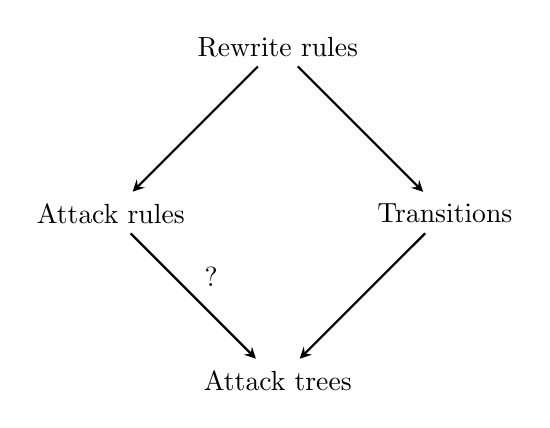
\begin{tikzpicture}[
    ->,
    >=stealth,
    shorten >=1pt,
    auto,
    thick,
    node distance=3cm
]
\node (rr) {Rewrite rules};
\node[below right of=rr] (t) {Transitions};
\node[below left of=rr] (ar) {Attack rules};
\node[below right of=ar] (at) {Attack trees};
\path
  (rr) edge (t)
  (rr) edge (ar)
  (ar) edge node {?} (at)
  (t) edge (at);
\end{tikzpicture}
  \caption{Relation between concepts on mvPDA and MTS}
  \label{fig:mvpda-mts-relation}
\end{figure}

Our goal is now to find a relation between attack rules and attack trees.
Figure \ref{fig:mvpda-mts-relation} shows the relation between different
concepts of PRS and MTS.  
For an mvPDA with a set of rewrite rules,
an MTS is induced with a set of transitions, from which
attack trees are induced.
Also from the rewrite rules, the attack rules are induced.
The missing connection is from attack rules to attack trees, which we need
to close.
For that, first we need show that there is a direct relation between transitions
and lifted versions of the transitions for an mvPDA.

\begin{lemma}
  \label{lemma:rule-lift}
  Given an MTS generated by a mvPDA,
  for $|p| ≥ 2$, $|q| ≥ 2$, $p,q$ sequential and any $s,t ∈ \mc P$:
\begin{align*}
  p \may[a] p' &\iff p⋅s \may[a] p'⋅s
  & &\text{and} &
  q \must[a] q' &\iff q⋅t \must[a] q'⋅t
\end{align*}
\end{lemma}
\begin{proof}
  \Rightarrow: Follows directly from the induction rules of an MTS from an mPRS.
  
  \Leftarrow: In the inference chain for $p⋅s \may[a] p'⋅s$,
  there is a $(r,a,r') ∈ \Dmay$ which was used to obtain that rule
  with $p⋅s = r⋅s'$ and $p'⋅s = r'⋅s'$. As $|r| ≤ |p|$, $|r'| ≤ |p'|$ and $p,p',r,r'$ are all
  sequential, there is $s''$ with $p = r⋅s''$ and $p' = r⋅s''$.
  Then we can infer the transition $r⋅s'' \may[a] r'⋅s'' = p \may[a] p'$.
  The same holds for $q⋅t \must[a] q'⋅t$.
\end{proof}

This can be applied to attack trees to lift their states
with added processes.

\begin{lemma}
  \label{lemma:tree-lift}
  Given an MTS induced by an mvPDA and any $s,t ∈ \mc P$:

  If there is an attack tree $T$ with $T_r = (p,q)$,
  then there is an attack tree $R$ with $R_r = (p⋅s, q⋅t)$ and
  $open(R) = \{ (p'⋅s,q'⋅t) \mid (p', q') ∈ open(T) \}$.
\end{lemma}
\begin{proof}
  In each base case in the construction of $T$, the
  attacking transition can be lifted with $s$ or $t$.
  For each defending transition, by lemma 
  \ref{lemma:rule-lift} there is exactly one lifted transition.
  Each other construction rule can still be applied on the
  lifted trees and we obtain the tree $R$.
\end{proof}

While attack rules are not powerful enough to represent any
attack tree, they can represent certain parts.
A part of a tree is essentially
a node with all edges and nodes to a set of ancestors,
while a partition is a disjunct union of parts resulting
in the complete tree.

\begin{definition}[Partition of an attack tree]
  A partition $\mathbb P$ of an attack tree $T$ is a set
  of subtrees $\mathbb P ⊆ subtree(T)$ with $T ∈ \mathbb P$.

  For $R_1,R_2 ∈ \mathbb P$, there is a partial ordering
  $R_1 ≤ R_2 \iff R_1 ∈ subtree(R_2)$ and consequently
  $R_1 < R_2 \iff R_1 ≤ R_2 ∧ R_1 ≠ R_2$.
  Under that relation, the partition successors of $R ∈ P$ given $\mathbb P$ are
  $succ_{\mathbb P}(R) = \{ R' ∈ \mathbb P \mid R' < R ∧ ¬∃ R'' : R' < R'' ∧ R'' < R \}$.
\end{definition}

An attack rule should then correspond to a part, or represent it, if
it can be lifted such that it leads from the root node of the part of
the part to all of its successors.

\begin{definition}[Part represented by an attack rule]
  A subtree $R ∈ \mathbb P$ in a partition
  is said to be \emph{represented} by an
  attack rule $(p,q) \attack S$ if there exist $s,t ∈ \mc P$
  such that $T_r = (p⋅s,q⋅t)$
  and $\{ R'_r \mid R' ∈ succ_{\mathbb P}(R) \} = \{ (p'⋅s,q'⋅t) \mid (p',q') ∈ S \}$
\end{definition}

Now we can prove our main theorem, allowing us
to decide existence of a closed tree by
using attack rules.

\begin{theorem}
  \label{theorem:tree-attack}
  For an mvPDA $(\Dmay, \Dmust)$ with its induced MTS $(\mc P, \may[], \must[])$,
  it holds that for any $P,S,Q,R ∈ Const$:
  \[
    ∃ T : T_r = (P⋅S,Q⋅R) ∧ closed(T) \iff (P⋅S,Q⋅T) \attack ∅
  \]
\end{theorem}
\begin{proof}
    \Rightarrow: Assume $T$ to be a closed tree with $T_r = (P⋅S,Q⋅R)$.

      First we show that if there is a partition $\mathbb P = \{T'_1, …, T'_n\}$
      of $T$ with $n$ elements
      such that each part is represented by an attack rule, then
      there is an attack rule $(P⋅S, Q⋅T) \attack ∅$.
      This is shown by induction on $n$:
      
      \begin{enumerate}
        \item $n = 1$: Then $P = \{T\}$ and there is a rule $(p,q) \attack S$
          representing $T$. As $(p⋅s,q⋅t) = T_r = (P⋅T,Q⋅R)$ and $|p| = |q| = 2$,
          necessarily $(p,q) = (P⋅T,Q⋅R)$ and as $succ_{\mathbb P}(T) = ∅$ it follows
          that $S = ∅$.
          Then the rule is $(P⋅T, Q⋅R) \attack ∅$.
        \item $n > 1$:
          For $T$ as the root part in $\mathbb P$,
          there is $T' ∈ succ_{\mathbb P}(T)$ as $n > 1$
          Let $T'_r = (p',q')$ and $(P⋅S,Q⋅R) \attack S$ be the rule representing $T$.
          We have $(p',q') ∈ S$ and necessarily $|p'| = |q'| ≥ 2$, as otherwise
          there would be no transition applicable from that state and
          therefore $T''$ would not exist. So the rule is a left-hand side rule.

          For every part $T'' ∈ {\mathbb P}$ with $succ_{\mathbb P}(T'') = ∅$,
          the representing rule $(p,q) \rightarrow S$ has $S = ∅$,
          so it is a right-hand side rule.
          Every path in $\mathbb P$ eventually leads to such a part.

          Then by following the successors of the parts from $T$ along the
          edges with $|p'| ≥ 2$ for the representing rule,
          eventually there will be a part $T'$ with a successor part $T''$ such that
          the rule representing $T'$ is a left-hand side rule and
          the rule representing $T''$ is a right-hand side rule.

          The partition $\mathbb P' = \mathbb P ∖ \{T''\}$ is again
          a partition of $T$
          where $succ_{\mathbb P'}(T') = succ_{\mathbb P}(T') ∖ \{T''\} ∪ succ_{\mathbb P}(T'')$ and
          other successors are unchanged.
          We now show that we can construct a rule representing $T'$ in $\mathbb P'$.

          Let $(p,q) \attack S$ be the rule representing $T'$ and
          $(p',q') \attack S'$ be the rule representing $T''$.
          By representation,
          there are $s,t ∈ \mc P$, $(p'',q'') ∈ S$ with $T''_r = (p''⋅s,q''⋅t)$ and
          $s',t' ∈ \mc P$ with $T''_r = (p'⋅s',q'⋅t')$.

          Then $(p''⋅s,q''⋅t) = (p'⋅s',q'⋅t')$.
          As $2 ≤ |p''| = |q''| ≤ 3$ and $|p'| = |q'| = 2$, either
          $s = s'$ and $t = t'$ or $P'⋅s = s'$ and $Q'⋅t = t'$ for some $P',Q' ∈ Const$.
          
          In the first case, we have $(p',q') = (p'',q'')$ and we can apply rule 3 to obtain
          $(p,q) \attack S ∖ \{(p'',q'')\} ∪ S'$.
          With $\{ (p'⋅s,q'⋅t) \mid (p',q') ∈ S ∖ \{(p'',q'')\} ∪ S' \} =
          \{ T'_r \mid succ_{\mathbb P'}(T') \}$,
          it represents $T'$ in $\mathbb P'$.

          In the second case, we have $(p'⋅P',q'⋅Q') = (p'',q'')$ and we can apply rule 4 to obtain
          $(p,q) \attack S ∖ \{(p'', q'')\} ∪ \{  (p''⋅P', q''⋅Q') \mid (p'',q'') ∈ S' \}$.
          With $\{ (p'⋅s,q'⋅t) \mid (p',q') ∈ S ∖ \{(p'',q'')\} \}$
          $∪ \{ (p''⋅P'⋅s,q''⋅Q'⋅t) \mid (p'',q'') ∈ S' \} =
          \{ T'_r \mid succ_{\mathbb P'}(T') \}$,
          it represents $T'$ in $\mathbb P'$.

          Then as $\mathbb P'$ is a partition for $T$ having a rule representing each part
          with $n - 1$ elements, we can apply the induction hypothesis and obtain
          the rule is $(P⋅T, Q⋅R) \attack ∅$.
      \end{enumerate}

      Now we need to show there is an initial partition for $T$ represented
      by attack rules.
      Take $\mathbb P = subtrees(T)$.
      For each $T' ∈ \mathbb P$,
      there is an attacking transition from $T'_r$ which induced $T'$.
      As $succ_P(T') = T'_C$, for each $T'' ∈ succ_P(T')$
      there is an appropriate defending transition to $T''_r$, and as
      $T'_O = ∅$ for each defending transition a $T'' ∈ succ_P(T')$ 

      Let $T'_t = (p⋅s,q⋅t)$ with $|p| = |q| = 2$ for some $s,t ∈ \mc P$.
      By lemma \ref{lemma:rule-lift}, for each transition
      $p⋅s \may[a] p'⋅s$ there is an inducing $(p, a, p') ∈ \Dmay$ and
      for each $q⋅t \may[a] q'⋅t$ there is an inducing $(q, a, q') ∈ \Dmay$.
      The same holds for $\must[a]$ and $\Dmust$.
      So there is a rule $(p, q) \attack \{ (p',q') \| (q, a, q') ∈ \Dmay \}$
      which represents $T'$.
    
    \Leftarrow:
      We show that if $(p,q) \attack S$, then there is a tree
      $T$ with $T_r = (p,q)$ such that $open(T) = S$
      by induction on the construction of $(p,q) \attack S$:
      \begin{enumerate}
        \item It was constructed by rule 1 from $(p, a, p') ∈ \Dmay$. Then there is
          an attacking transition $p \may[a] p'$ and 
          for every $(q, a, q') ∈ \Dmay$ there is an induced defending transition
          $q \may[a] q'$.
          Then $S = \{ (p',q') | q \may[a] q' \}$ and by attack tree inference rule 1
          there is $T = ((p, q), S, ∅)$ with $open(T) = S$.
        \item It was constructed by rule 2 from $(q, a, q') ∈ \Dmust$. Then there is
          an attacking transition $q \must[a] q'$ and 
          for every $(p, a, p') ∈ \Dmust$ there is an induced defending transition
          $p \must[a] p'$.
          Then $S = \{ (p',q') | p \must[a] p' \}$ and by attack tree inference rule 2
          there is $T = ((p, q), S, ∅)$ with $open(T) = S$.
        \item It was constructed by rule 3 from
          $(p,q) \attack S'' \uplus \{(p',q')\} $ and
          $(p',q') \attack S'$ with $S = S'' ∪ S'$.
          Then by induction hypothesis there is
          a tree $T'$ with $T'_r = (p',q')$ and $open(T') = S'$ and
          a tree $T''$ with $T''_r = (p,q)$ and $open(T'') = S'' \uplus \{(p',q')\}$.
          By applying lemma \ref{lemma:tree-composition} on $T'$ and $T''$ there is
          a tree $T$ with $T_r = (p,q)$ with $open(T) = S'' ∪ S' = S$.
        \item It was constructed by rule 4 from
          $(p,q) \attack S'' \uplus \{(p'⋅P,q'⋅Q)\}$ and
          $(p',q') \attack S'$ with $S = S'' ∪ S'''$ and
          $S''' = \{  (p''⋅P, q''⋅Q) \mid (p'',q'') ∈ S' \}$.
          Then by induction hypothesis there is
          a tree $T'$ with $T'_r = (p',q')$ and $open(T') = S'$ and
          a tree $T''$ with $T''_r = (p,q)$ and $open(T'') = S'' \uplus \{(p'⋅P,q'⋅Q)\}$.
          By applying lemma \ref{lemma:tree-lift} on $T'$ there is a tree
          $T'''$ with $T'''_r = (p'⋅P,q'⋅Q)$,
          $open(T''') = O''' \uplus \{(p'⋅P,q'⋅Q)\}$ and
          $O''' = \{ (p''⋅P, q''⋅Q) \mid (p'',q'') ∈ S' \} = S'''$.
          By applying lemma \ref{lemma:tree-composition} on $T''$ and $T'''$ there is
          a tree $T$ with $T_r = (p,q)$ and $open(T) = S'' ∪ S''' = S$.
      \end{enumerate}
      Therefore if $(P⋅S,Q⋅R) \attack ∅$, then there is a tree
      $T$ with $T_r = (P⋅S,Q⋅R)$ and $open(T) = ∅$.
\end{proof}

\begin{example}

  Again we regard the vending machine mvPDA from figure \ref{fig:vending-mvpda}.
  We will see how to derive the attack tree from figure
  \ref{fig:vending-combined-attack-tree} with attack rules to prove that
  $P⋅S ≤_m Q⋅S$ does not hold.

\begin{figure}[ht]
  \centering
\begin{tikzpicture}[
  level 1/.style={level distance=1.5cm, sibling distance=2cm},
  edge from parent path={(\tikzparentnode.east) -- (\tikzchildnode.west)},
]
  \node[state] (R1) {$(P⋅S,Q⋅S) \attack[] \{ (P⋅M⋅S,Q⋅C⋅S), (P⋅M⋅S,Q⋅T⋅S) \}$};
  \node[attlabel, left of=R1] {$T_1$};
  
  \node[state, below of=R1, node distance=1cm] (R2) {$(P⋅M,Q⋅T) \attack[] \{ (P⋅M⋅M,Q⋅T⋅T) \}$};
  \node[attlabel, left of=R2] {$T_2$};

  \node[state, below of=R2, node distance=1cm] (R3) {$(P⋅M,Q⋅C) \attack[] \{ (P⋅M⋅M,Q⋅C⋅C) \}$};
  \node[attlabel, left of=R3] {$T_3$};

  \node[state, below of=R3, node distance=1cm] (R4) {$(P⋅M,Q⋅T) \attack[] \{ (C,Q) \} $};
  \node[attlabel, left of=R4] {$T_4$};

  \node[state, below of=R4, node distance=1cm] (R5) {$(P⋅M,Q⋅C) \attack[] \{ (T,Q) \} $};
  \node[attlabel, left of=R5] {$T_5$};
  
  \node[state, below of=R5, node distance=1cm] (R6) {$(C⋅M,Q⋅T) \attack[] ∅$};
  \node[attlabel, left of=R6] {$T_6$};
  
  \node[state, below of=R6, node distance=1cm] (R7) {$(T⋅M,Q⋅C) \attack[] ∅$};
  \node[attlabel, left of=R7] {$T_7$};
\end{tikzpicture}
  \caption{Attack rules for first partition of vending machine tree}
  \label{fig:vending-attackrule-tree-1}
\end{figure}


\begin{figure}[ht]
  \centering
\begin{tikzpicture}[
  level 1/.style={level distance=1.5cm, sibling distance=2cm},
  edge from parent path={(\tikzparentnode.east) -- (\tikzchildnode.west)},
]
  \node[state] (R1) {$(P⋅S,Q⋅S) \attack[] \{ (P⋅M⋅S,Q⋅C⋅S), (P⋅M⋅S,Q⋅T⋅S) \}$};
  \node[attlabel, left of=R1] {$T_1$};
  
  \node[state, below of=R1, node distance=1cm] (R2) {$(P⋅M,Q⋅T) \attack[] \{ (C⋅M,Q⋅T) \}$};
  \node[attlabel, left of=R2] {$T_2$}
  child {
    node {$T_4$}
  };

  \node[state, below of=R2, node distance=1cm] (R3) {$(P⋅M,Q⋅C) \attack[] \{ (T⋅M,Q⋅C) \}$};
  \node[attlabel, left of=R3] {$T_3$}
  child {
    node {$T_5$}
  };
  
  \node[state, below of=R3, node distance=1cm] (R6) {$(C⋅M,Q⋅T) \attack[] ∅$};
  \node[attlabel, left of=R6] {$T_6$};
  
  \node[state, below of=R6, node distance=1cm] (R7) {$(T⋅M,Q⋅C) \attack[] ∅$};
  \node[attlabel, left of=R7] {$T_7$};
\end{tikzpicture}
  \caption{Attack rules for second partition of vending machine tree}
  \label{fig:vending-attackrule-tree-2}
\end{figure}

  Initially we take the first partition of the attack tree, where every
  part has a basic attack rule representing it, as shown in figure 
  \ref{fig:vending-attackrule-tree-1}.
  Note that the rules from $T_1$, $T_2$, and $T_3$ are left-hand side rules
  and the rules from $T_4$, $T_5$, $T_6$, $T_7$ are right-hand side rules.
  So the only rules we can combine are the ones from $T_2$ with $T_4$ and
  $T_3$ with $T_5$. Then we obtain the second partition and rules shown in
  figure \ref{fig:vending-attackrule-tree-2}.

\begin{figure}[ht]
  \centering
\begin{tikzpicture}[
  level 1/.style={level distance=1.5cm, sibling distance=2cm},
  level 2/.style={level distance=1.5cm, sibling distance=2cm},
  edge from parent path={(\tikzparentnode.east) -- (\tikzchildnode.west)},
]
  \node[state] (R1) {$(P⋅S,Q⋅S) \attack[] \{ (P⋅M⋅S,Q⋅C⋅S), (P⋅M⋅S,Q⋅T⋅S) \}$};
  \node[attlabel, left of=R1] {$T_1$};
  
  \node[state, below of=R1, node distance=1cm] (R2) {$(P⋅M,Q⋅T) \attack[] ∅ \}$};
  \node[attlabel, left of=R2] {$T_2$}
  child {
    node {$T_4$}
    child {
      node {$T_6$}
    }
  };

  \node[state, below of=R2, node distance=1cm] (R3) {$(P⋅M,Q⋅C) \attack[] ∅$};
  \node[attlabel, left of=R3] {$T_3$}
  child {
    node {$T_5$}
    child {
      node {$T_7$}
    }
  };
\end{tikzpicture}
  \caption{Attack rules for third partition of vending machine tree}
  \label{fig:vending-attackrule-tree-3}
\end{figure}

  After that we can combine the rules from $T_2$ with $T_6$ and from $T_3$
  with $T_7$. This results in the third partition and rules shown in
  figure \ref{fig:vending-attackrule-tree-3}.
  Finally we combine $T_1$ first with $T_2$ and then with $T_3$ to obtain
  the fourth partition with the rule shown in figure \ref{fig:vending-attackrule-tree-4}.
  This partition represents the whole tree, and as $(P⋅S, Q⋅S) \attack ∅$, we
  can decide that there is a winning strategy from $(P⋅S, Q⋅S)$,
  therefore the states do not refine.

\begin{figure}[ht]
  \centering
\begin{tikzpicture}[
  level 1/.style={level distance=1.5cm, sibling distance=2cm},
  level 2/.style={level distance=1.5cm, sibling distance=2cm},
  level 3/.style={level distance=1.5cm, sibling distance=2cm},
  edge from parent path={(\tikzparentnode.east) -- (\tikzchildnode.west)},
]
  \node[state] (R1) {$(P⋅S,Q⋅S) \attack[] ∅$};
  \node[attlabel, left of=R1] {$T_1$}
  child {
    node {$T_3$}
    child {
      node {$T_5$}
      child {
        node {$T_7$}
      }
    }
  }
  child {
    node {$T_2$}
    child {
      node {$T_4$}
      child {
        node {$T_6$}
      }
    }
  };
\end{tikzpicture}
  \caption{Attack rules for fourth partition of vending machine tree}
  \label{fig:vending-attackrule-tree-4}
\end{figure}

\end{example}

